%%%%%%%%%%%%%%%%%%%%%%%%%%%%%%%%%%%%%%%%%
% Journal Article
% LaTeX Template
% Version 1.4 (15/5/16)
%
% This template has been downloaded from:
% http://www.LaTeXTemplates.com
%
% Original author:
% Frits Wenneker (http://www.howtotex.com) with extensive modifications by
% Vel (vel@LaTeXTemplates.com)
%
% License:
% CC BY-NC-SA 3.0 (http://creativecommons.org/licenses/by-nc-sa/3.0/)
%
%%%%%%%%%%%%%%%%%%%%%%%%%%%%%%%%%%%%%%%%%

%----------------------------------------------------------------------------------------
%	PACKAGES AND OTHER DOCUMENT CONFIGURATIONS
%----------------------------------------------------------------------------------------

\documentclass[twoside,twocolumn]{article}

\usepackage{blindtext} % Package to generate dummy text throughout this template 

\usepackage[sc]{mathpazo} % Use the Palatino font
\usepackage[T1]{fontenc} % Use 8-bit encoding that has 256 glyphs
\linespread{1.05} % Line spacing - Palatino needs more space between lines
\usepackage{microtype} % Slightly tweak font spacing for aesthetics
\usepackage[pdftex]{graphicx}    
\usepackage{units}
\usepackage{amsmath}
\usepackage{breqn}
\usepackage{listings}    
\usepackage[spanish]{babel}
\usepackage[utf8]{inputenc}

\usepackage[hmarginratio=1:1,top=32mm,columnsep=20pt]{geometry} % Document margins
\usepackage[hang, small,labelfont=bf,up,textfont=it,up]{caption} % Custom captions under/above floats in tables or figures
\usepackage{booktabs} % Horizontal rules in tables

\usepackage{lettrine} % The lettrine is the first enlarged letter at the beginning of the text

\usepackage{enumitem} % Customized lists
\setlist[itemize]{noitemsep} % Make itemize lists more compact
\AtBeginDocument{%
  \renewcommand\tablename{Tabla}
}
\usepackage{abstract} % Allows abstract customization
\renewcommand{\abstractnamefont}{\normalfont\bfseries} % Set the "Abstract" text to bold
\renewcommand{\abstracttextfont}{\normalfont\small\itshape} % Set the abstract itself to small italic text
\setlength\parindent{0pt}
\usepackage{titlesec} % Allows customization of titles
\renewcommand\thesection{\Roman{section}} % Roman numerals for the sections
\renewcommand\thesubsection{\roman{subsection}} % roman numerals for subsections

\titleformat{\section}[block]{\large\scshape\centering}{\thesection.}{1em}{} % Change the look of the section titles
\titleformat{\subsection}[block]{\large}{\thesubsection.}{1em}{} % Change the look of the section titles
\usepackage{xcolor}
\definecolor{light-gray}{gray}{0.95}
\newcommand{\code}[1]{\colorbox{light-gray}{\texttt{#1}}}
\usepackage{fancyhdr} % Headers and footers
\pagestyle{fancy} % All pages have headers and footers
\fancyhead{} % Blank out the default header
\fancyfoot{} % Blank out the default footer
\fancyhead[C]{Propagación de una Epidemia mediante Autómatas Celulares$\bullet$ Noviembre 2016 $\bullet$ Herramientas Computacionales} % Custom header text
\fancyfoot[RO,LE]{\thepage} % Custom footer text

\usepackage{titling} % Customizing the title section
\usepackage{float}
\usepackage{hyperref} % For hyperlinks in the PDF

%----------------------------------------------------------------------------------------
%	TITLE SECTION
%----------------------------------------------------------------------------------------

\setlength{\droptitle}{-4\baselineskip} % Move the title up

\pretitle{\begin{center}\Huge\bfseries} % Article title formatting
\posttitle{\end{center}} % Article title closing formatting
\title{Propagación de una Epidemia mediante Autómatas Celulares} % Article title
\author{%
\textsc{Julián Jiménez Cárdenas} \\[1ex] % Your name
\normalsize \href{mailto:juojimenezca@unal.edu.co}{juojimenezca@unal.edu.co} % Your email address
\and % Uncomment if 2 authors are required, duplicate these 4 lines if more
\textsc{Juan Sebastián Ordóñez Soto} \\[1ex]
\normalsize \href{mailto:jsordonezs@unal.edu.co}{jsordonezs@unal.edu.co} 
% Your email address
\\ \\ \normalsize{Herramientas Computacionales, Departamento de Física, Universidad Nacional, Bogotá.} % Your institution
}

\date{\normalsize{Noviembre 29, 2016}} % Leave empty to omit a date
\renewcommand{\maketitlehookd}{%
\begin{abstract}
\normalsize{En el presente artículo se muestran los resultados obtenidos al reproducir el algoritmo descrito en \cite{b1}, en éste los autores buscaban simular la evolución de una epidemia mediante difusión utilizando un objeto llamado \emph{Autómatas Celulares}, con acciones bien definidas (reglas de evolución) en cierto intervalo de tiempo. Asimismo, se comprueba la validez del método al compararlo con el modelo \textbf{SIR}, comúnmente utilizado en el modelamiento de este fenómeno.}
\end{abstract}
}


%----------------------------------------------------------------------------------------

\begin{document}
\maketitle
\section{Introducción al Problema}
El objetivo de la simulación es reproducir el comportamiento temporal de una epidemia por difusión mediante autómatas celulares. Para ello, deben estar ubicados en un mismo punto al principio de la simulación y después irse moviendo a lo largo del espacio previamente discretizado.\\ \\
Referente al autómata celular, es un objeto (en este caso, una estructura de \code{C++}) regido por reglas de evolución simples descritas en la subsección \textit{Algoritmo}. Las variables determinantes para simular el comportamiento son: el número de autómatas celulares $N$, la probabilidad que tiene un autómata infectado de curarse $PInm$, el tamaño de la malla bidimensional en la que estarán los autómatas, el número inicial de infectados, la probabilidad de que un autómata se infecte por la presencia de autómatas infectados $r$ y el tiempo de evolución del sistema (en unidades arbitrarias).\\ \\
Después de reproducir los resultados del modelo \textbf{SIR}, se analizaron algunos casos de prueba, así como la relación existente entre la probabilidad de volverse inmune siendo infectado $PInm$ contra el número final de autómatas susceptibles.
\subsection{Algoritmo}
Los autómatas celulares fueron programados para seguir las siguientes reglas. En cada paso de tiempo se deben realizar las siguientes acciones.
\subsubsection{Movimiento Difusivo}
\begin{enumerate}
\item La célula rotará con igual probabilidad hacia arriba, abajo, derecha o izquierda.
\item La célula se moverá en la dirección a la cual apunta. Hay que tener precaución, pues la célula no se debe salir de los límites del mapa.
\end{enumerate}
\subsubsection{Contagio Epidémico}
\begin{enumerate}
\item Si la célula está inmune sigue inmune.
\item Si está infectada se cura con probabilidad $PInm$.
\item Si está sano y tiene infectados en el mismo punto o a sus alrededores, se calcula la probabilidad que éste tiene de infectarse proporcionalmente al número de infectados alrededor suyo. Mediante dicha probabilidad se determinará si se infecta la célula o no.
\end{enumerate}
Cabe hacer énfasis en que las celdas en las que se ubican los autómatas celulares y éstos son distintos.

\section{Código}
Los programas encargados de calcular el comportamiento de los autómatas celulares se hicieron en \code{C++}. De éstos se generaban archivos de texto plano, para ser posteriormente leídos y relacionados mediante scripts de \code{Python}. En aras de generar números aleatorios en \code{C++}, se usó la librería \code{random} y el generador \code{mt19937}. Con estas herramientas se creó una función para determinar si (pseudo-aleatoriamente) se da un evento con cierta probabilidad.\\ \\
También se aplicaron las librerías \code{stdio} y \code{fstream}, para mostrar información por consola e imprimir los datos en un archivo de texto, respectivamente. Todos los datos fueron almacenados en arreglos simples de \code{C++}, y, como ya se había comentado, se implementó la estructura \code{Cell} con los atributos necesarios, con el fin de evitar \textit{cache missings}.\\ \\
Los códigos se ejecutaron en un \textit{HP ENVY 15 Notebook PC}, con \textit{Intel Corporation Xeon E3-1200 v3/4th Gen Core Processor}, con RAM de 12GB, desde Ubuntu 16.04.\\ \\
La cantidad de iteraciones usadas para cada $PInm$ es 50. El comportamiento correspondiente al \textbf{SIR} se aprecia a plenitud normalmente en las primeras 10 iteraciones.\\ \\
Respecto al código en \code{Python}, se usó \code{numpy} para leer el archivo de texto generado anteriormente y \code{matplotlib} para realizar las respectivas gráficas.\\ \\
Durante el testeo del programa, se notó que, en principio, tardaba mucho. Por ende, se usó \code{gprof} para determinar cuáles partes del código estaban mal optimizadas. Puntualmente, en la función \code{howManyInf} (encargada de obtener el número de infectados alrededor de un célula sana), se mejoraron las condiciones para ver cuántas células infectadas hay alrededor de las sanas, con lo cual se disminuyó notablemente el tiempo de ejecución.
\section{Análisis y Resultados}
\subsection{Casos de Prueba}
Para corroborar que el algoritmo del código estuviera bien planteado, se plantearon casos de prueba, mostrados a continuación.
\subsubsection{$pInm=1$}
En este primer caso, se espera ver que una pequeña parte de la población susceptible se infecte y se vuelva inmune rápidamente, es decir, una disminución mínima en $S$ hasta un valor constante y de forma similar, un aumento mínimo en $R$. Para los $I$ el cambio es imperceptible, pues su población inicial es muy pequeña y pasa a ser nula en pocas iteraciones.
\begin{figure}[H]
\begin{center}
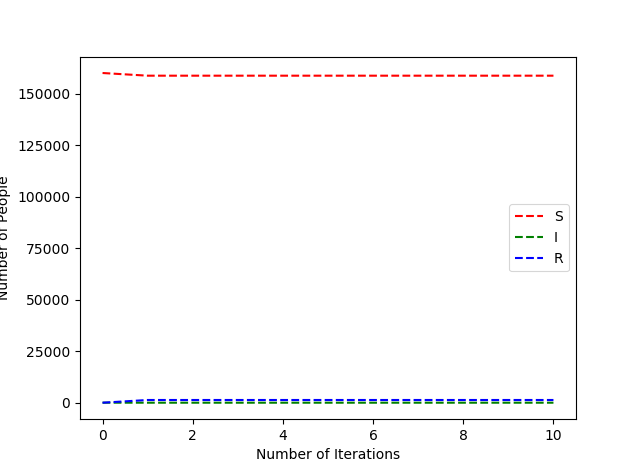
\includegraphics[width=.5\textwidth]{Pinm1}
\caption{Gráfica con la probabilidad de inmunizarse ($pInm$) igual a 1}
\end{center}
\end{figure}
\subsubsection{$pInm=0$}
Para este segundo caso, se espera que toda la población llegue a ser infectada, por lo tanto, la población $S$ decrece en un par de iteraciones y asimismo la población $I$ crece; mientras tanto, $R$ permanece constante e igual a cero, pues nadie se cura. 
\begin{figure}[H]
\begin{center}
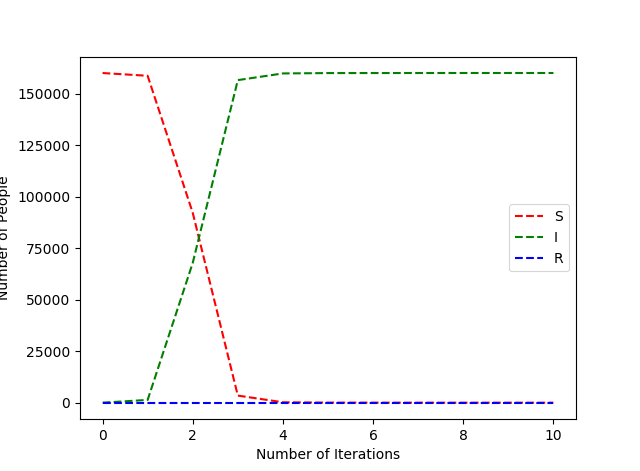
\includegraphics[width=.5\textwidth]{0Pinm}
\caption{Gráfica con la probabilidad de inmunizarse ($pInm$) igual a 0}
\end{center}
\end{figure}

\subsection{$pInm=0.4$ y $r=0.00218$}
Este caso es el que recrean en \cite{b1}, mostrando la validez de este método con el modelo \textbf{SIR}. Para obtener esta gráfica, se corrió el programa seis veces con una semilla diferente determinada en cada ocasión.
\begin{figure}[H]
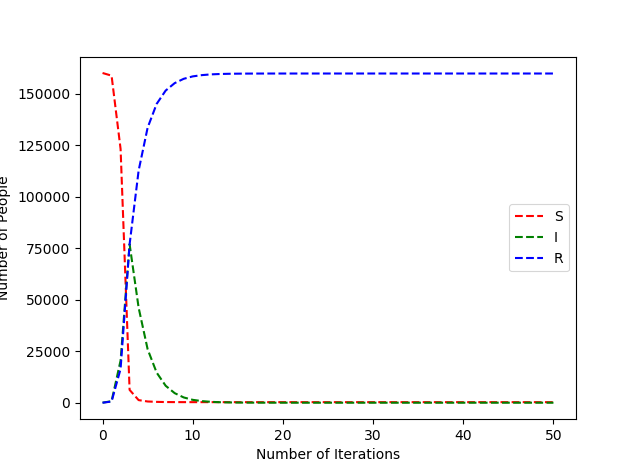
\includegraphics[width=.5\textwidth]{IterationsVSNumber}
\caption{Relación entre el número de iteraciones y \textbf{SIR}}
\end{figure}
\subsection{Relación entre $pInm$ y el número final de susceptibles}
Para las simulaciones hasta 50 iteraciones, se comprobó una ley exponencial. Este resultado es reproducible independientemente del número de iteraciones, pues hay un leve período en el cual se produce un contagio notable; cuando las células se encuentran cerca unas de otras. La evolución posterior depende de la primera parte de la misma.
\begin{figure}[H]
\begin{center}
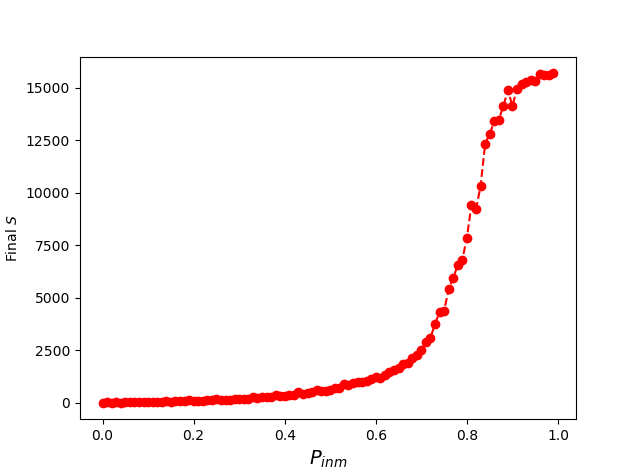
\includegraphics[width=.5\textwidth]{PinmVSs}
\end{center}
\caption{Relación entre la probabilidad de inmunización y la cantidad de susceptibles final (después de 50 iteraciones)}
\label{First}
\end{figure} 
Además, si suponemos que la relación se rige por un comportamiento tipo exponencial (notable al hacer la gráfica \ref{First} en semi-logarítmico), es decir, $S=a^{pI_{nm}}$, al calcular el valor de la pendiente, se obtiene que $a=11.4030158925$.
\begin{figure}[H]
\begin{center}
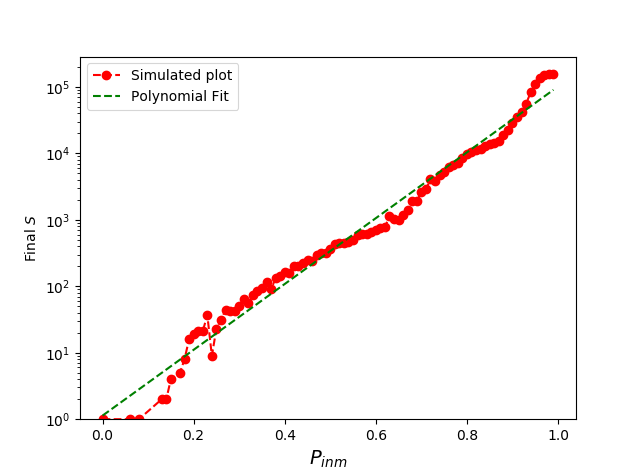
\includegraphics[width=.5\textwidth]{PinmVSsSemilog.png}
\end{center}
\caption{Relación entre la probabilidad de inmunización y la cantidad de susceptibles final (después de 50 iteraciones) en semi-logarítmico con su respectivo arreglo lineal} 
\end{figure}

\section{Conclusiones}
\begin{enumerate}
\item Mediante las herramientas computacionales se pueden resolver problemas que, matemáticamente suelen ser más complejos de tratar, como el modelo \textbf{SIR}. Además, es posible implementar elementos, en otro modo imposible, como por ejemplo, características demográficas.

\item Realizando la gráfica semi-logarítmica, se obtiene una ley exponencial que relaciona la probabilidad de inmunización $pInm$ con la cantidad de susceptibles final, con coeficiente $a=11.4030158925$. 
\end{enumerate}
\begin{thebibliography}{99} % Bibliography - this is intentionally simple in this template

%\bibitem[Figueredo and Wolf, 2009]{Figueredo:2009dg}
%Figueredo, A.~J. and Wolf, P. S.~A. (2009).
%\newblock Assortative pairing and life history strategy - a cross-cultural
%  study.
%\newblock {\em Human Nature}, 20:317--330.
\bibitem[1]{b1}W. F. Oquendo y J. D. Muñoz.  \emph{Simulación de la Propagación de una Epidemia Utilizando un Autómata Celular de Difusión Bidimensional}; Revista Colombiana de Física, Vol40, No.2, Julio 2008.

\end{thebibliography}
\end{document}